\newpage
\section{Aufbau und Durchführung}
\label{sec:Durchführung}
\paragraph{Justage}
In der Abbildung \ref{fig:aufbau} ist
der Versuchsaufbau dargestellt.
\begin{figure}
  \centering
  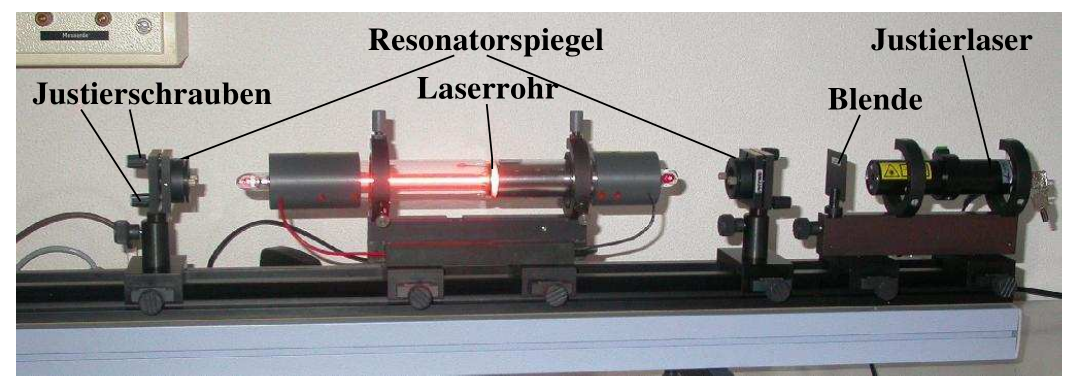
\includegraphics[width=0.7\textwidth]{figures/Aufbau.PNG}
  \caption{Versuchsaufbau.}
  \label{fig:aufbau}
\end{figure}
Bevor jedoch mit den eigentlichen Messungen
begonnen werden
kann, muss eine Justage der Bauteile auf der optischen Bank vorgenommen werden.
Zunachst wird der Justagelaser auf die optische Achse
ausgerichtet
mit Hilfe eines Schirm mit Fadenkreuz und Beugungsblende
ausgerichtet.
Dann wird der Austritts Resonatorspiegel
auf die optischen Bank plaziert
und mit den Justierschrauben so ausgereichtet,
dass die erste Reflektion wieder auf die
Mitte des Fadenkreuz tifft.
Danach wird der
zweite Resonatorspiegel zwischen Justagelaser
und erstem Spiegel plaziet.
Diesmal wird die zweite Reflektion
auf das Fadenkreuz ausgereichtet.
Jetzt kann die Laserröhre mit dem Helium-Neon-Gasgemisch und
den beiden Brewster-Fenster am Ausgang
zwischen beiden Resonatorspiegeln
plaziert werden.
Dann wird der Justierlaser abgeschaltet
und ein Strom an die
Elektroden in der Laserröhre
angelegt, sodass mittels Entladung eine Inversion
stattfindet. Bei korrekter
Justage setzt die Lasertätigkeit direkt ein
und es bildet sich ein Laserstrahl
zwischen den Resonatorspiegeln aus.
Falls nicht muss an den Justierschrauben
nachträglich justiert werden.
Der Laserstrahl tritt nun aus dem OC(out coupling) Resonatorspiegel
aus und die Intensität wird mit einer Photodiode gemessen.
Die Intensität wird durch Nachjustiern der Schrauben maximiert und
es kann mit den Messungen begonnen werden.



\paragraph{Durchführung}
\paragraph{ Untersuchung der Polarisation}
Zunächst wird die Polarisation des Helium-Neon-Lasers
untersucht. Dafür wird hinter dem OC Spiegel ein
Polarisationsfilter auf der optischen Bank
plaziert und dessen Winkel varriert. Mit Hilfe einer Photodiode wird
die Intensität des Laserstrahls in Abhängigkeit des Winkels gemessen.

\paragraph{Bestimmung der Wellenlänge}
Die Wellenlänge des HeNe-Lasers wird mit zwei unterschiedlichen
Gittern durch ein Beugungsexperiment aus Schirmabstand
und den Abständen der Beugungsmaxima zum Hauptmaximum bestimmt.

\paragraph{Unterschuchung der TEM-Moden}
Zunächst werden die longitudinalen Moden untersucht. Dafür
wird die Resonatorlänge variert und das Frequenzspektrum des Laser
mit einem Frequenzspektrometer aufgenommen.
Falls bei der Variation der Resonatorlänge die Lasertätigkeit
nachlässt, muss mit den Justierschrauben nachgeregelt werden.

Dann werden bei fester Resonatorlänge zwei transversale Moden untersucht.
Dafür wird zunächst die $\text{TEM}_{00}$, untersucht indem hinter dem
Laser eine defokussierende Linse plaziert wird und mit Hilfe einer
Photodiode auf einer Schiebebank die Intensitätsverteilungen
durchgemessen werden.
Für die $\text{TEM}_{01}$ wird zwischen den beiden Resonatorspiegeln
ein dünner Wolframdraht plaziert. Bei genauer Plazierung kann so auf
einem Schirm die gewünschte Mode beobachtet
und wieder Vermessen werden.


\paragraph{Überprüfung der Stabilitätsbedingung}
Um die Stabilitätsbedingung zu überprüfen
wird die Resonatorlänge varriert und jeweils
die Laserleistung durch nachjustiern maximiert und in Abhängigkeit von
der Länge gemessen.
